\vspace{-4mm}

\section{Introduction}

\label{sec:introduction}

\vspace{-2mm}

\begin{wrapfigure}{r}{0.6\textwidth}
\vspace{-6mm}
    \begin{center}
    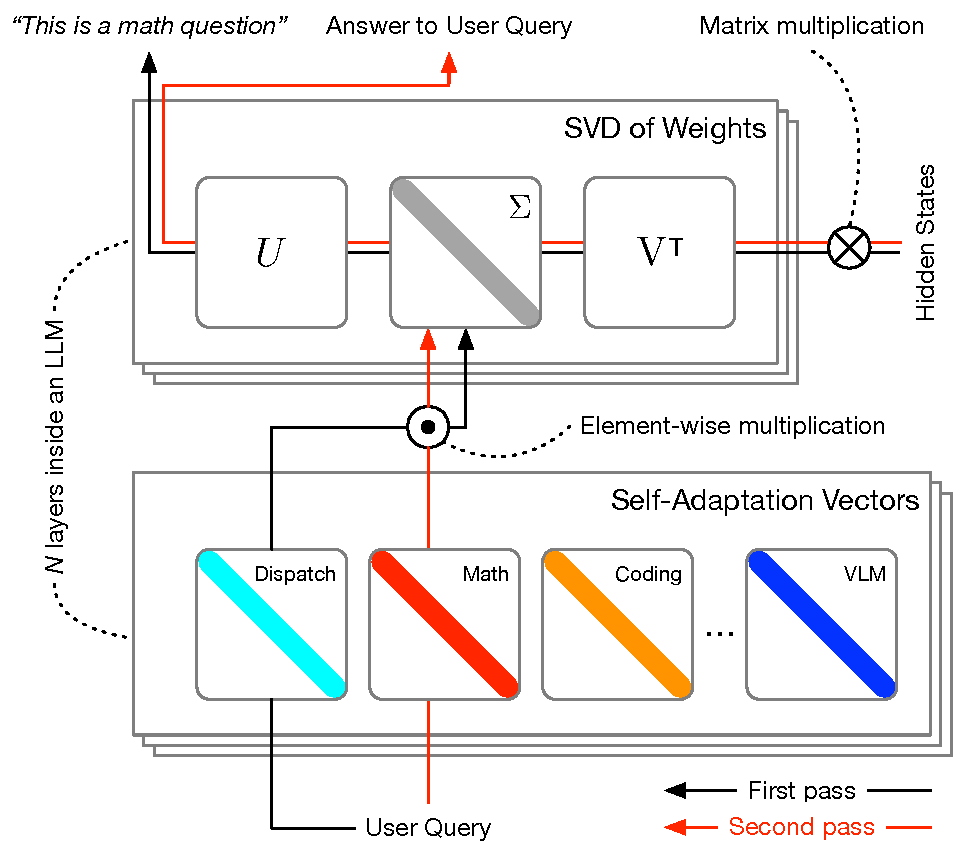
\includegraphics[width=0.6\textwidth,height=0.4\textwidth,keepaspectratio]{images/cover.pdf}
    \end{center}
  \vspace{-4mm}
  \caption{\textbf{Overview of \implname.} In the training phase, we tune the scales of the singular values of the weight matrices to generate a set of ``expert'' vectors, each of which specializes in one type of tasks. In the inference phase, a two-pass process is adopted where the first applies the task-specific expert and the second generates the answer.}
  \label{fig:cover}
  \vspace{-4mm}
\end{wrapfigure}

Self-adaptive large language models (LLMs) would represent a significant advancement in artificial intelligence, providing a framework where models can adjust to varied tasks and dynamic contexts in real time.
While compositionality and scalability are crucial for effective adaptation, current LLM training methodologies fall short of achieving both these properties simultaneously.
Our research aims to present a pioneering solution to realize this vision and address these gaps.

Traditionally, LLM post-training has sought to optimize a model for a wide range of capabilities in a single, extensive training session.
While this ``one-shot’’ fine-tuning framework is ideal from a simplicity perspective, it is also difficult to achieve in practice.
For instance, post-training is still highly resource-intensive, leading to significant computational costs and training times.
Additionally, there tends to be notable performance trade-offs when introducing additional breadth to the data, making it challenging to overcome overfitting and task interference at the same time.

In contrast, self-adaptive models offer a more flexible and efficient approach.
Rather than attempting to train an LLM for all tasks in one step, expert modules can be developed offline and augmented to the base LLM on-demand~\citep{kang2024self}.
This allows the model to dynamically modify its behavior based on the task at hand, without the need for constant re-tuning.
In addition to the benefit of having independent components, this modularity also supports continual learning, enabling the model to add new skills over time without catastrophic forgetting.
Moreover, self-adaptive LLMs mirror a well-established principle in neuroscience and computational biology, where the brain activates specific regions depending on the task at hand~\citep{loose2017switch} and dynamically reconfigures its functional networks in response to changing task demands~\citep{davison2015brain}.

In principle, the first step toward achieving self-adaptive LLMs can be realized through the development of specialized expert modules, each fine-tuned~\citep{kaplan2020scaling} via techniques such as low-rank adaptation (LoRA)~\citep{hu2021lora}.
These expert modules can then be dynamically composed at runtime based on the task demands, a process that can be efficiently managed through Mixture of Experts (MoE)-like systems~\citep{ICML2024_MoE}.
However, several challenges need to be addressed to make this approach both scalable and compositional.
First, fine-tuning LLMs to create multiple expert modules significantly increases the number of parameters that need to be trained.
In practice, even with parameter-efficient methods like LoRA, the cumulative size of these modules can quickly escalate, leading to increased storage and computational demands.
Second, these expert modules are often prone to overfitting, a phenomenon especially prevalent when training on smaller datasets or narrow task domains.
Third, the flexible composition of these expert modules also presents largely unresolved challenges currently posing as open research problems. 

To overcome these limitations, we first propose \svdname (\svdacro), a novel parameter-efficient fine-tuning (PEFT) method to obtain effective building blocks for self-adaptation.
\svdacro works by extracting and tuning only the singular values within the model's weight matrices.
By focusing on this principled parameterization, our approach mitigates the risk of overfitting, drastically reduces computational demands, and allows for inherent compositionality.
We show these properties enable us to cheaply obtain a set of effective domain-specific ``expert’’ vectors by training on narrow datasets with RL, directly optimizing task performance on individual topics.

We then introduce our full \implname framework to empower LLMs through the underlying principles of self-adaptation.
Given a prompt from an unknown task, \implname entails a two-pass inference mechanism which we illustrate in Figure~\ref{fig:cover}.
During the first pass, \implname executes the model and observes its test-time behavior, gathering the relevant information to understand the necessary skills to tackle the current problem.
During the second pass, our framework uses this information to combine the available expert vectors and provide a new modification to the base weights of the LLM specifically tailored to its test-time conditions. 
We design three different adaptation strategies that can be used within \implname, which we show provide monotonic performance benefits with increasing access to the test-time conditions.

We evaluate \svdacro and the full \implname framework through extensive experiments across a diverse range of LLMs and tasks.
First, when trained on domain-specific datasets, we show that \svdacro consistently outperforms traditional strategies for efficient fine-tuning such as LoRA, and at the same time, with orders of magnitudes fewer parameters.
Then we show that \implname is able to push performance far further, effectively adapting the weights of the base model even in entirely out-of-distribution applications such as visual question answering.
Finally, we analyze the properties of our new framework, validating that it provides increasing benefits with additional access to its current test-time conditions and even allow for recycling pre-trained \svdacro experts across model architectures.
In summary, our key technical contributions are the following: 
\begin{itemize}
\item The development of \implname as a pivotal self-adaptation framework for LLMs, providing a universal blueprint to dynamically adapt the behavior of LLMs from a growing set of pre-trained skills.
\item The introduction of \svdacro, a novel PEFT method trainable with RL on small datasets, producing compact expert vectors with inherent compositionality, all key properties necessary for our scalable self-adaptation framework.
\item The implementation of three adaptation strategies within \implname, effectively dispatching \svdacro-trained experts with properties designed to cope with different requirements and deployment scenarios.
\end{itemize}
